%!TEX root = chi14grammatical.tex
Our results imply that auto-suggest interfaces for syntactic search should show candidate relationships augmented with a list of phrases in which they occur. A list of phrases is the most recognizable presentation for clausal relationships, and is as good as a list of words for the other types of relations. A mockup of such a search box is shown in Figure \ref{fig:phrases-mockup}.
\begin{figure}
\centering
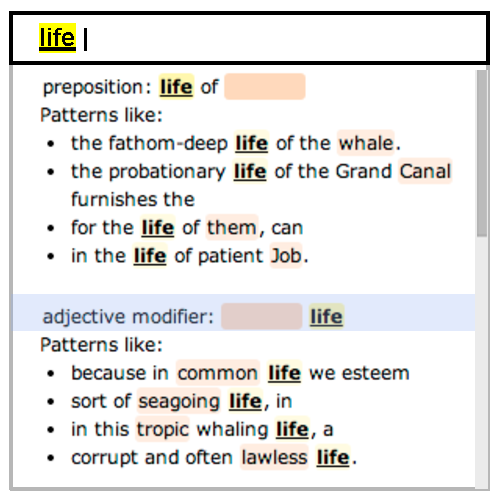
\includegraphics[width=0.5\columnwidth]{fig/phrases-mockup}
\caption{
	\label{fig:phrases-mockup} Mockup of auto-suggest for syntactic search on the word `life', showing the most common grammatical relations with example phrases for each.
}
\end{figure}

